\section{Getting started}

The core of any distpy project is the same basic python script.
This has been designed so that transferrable parallel processing workflows a possible across Windows and Linux environments, so we'll
give details as to the design choices made.
You can of course depart from this template in your own projects, this example serves as a starting point.

\subsection{python  example}
\begin{lstlisting}
# ingest data from an archived data store to a hot or scratch space
import distpy.ingesters.parallel_ingest_sgy
# apply a signal processing flow, resulting in new results to the scratch space or archive
import distpy.controllers.parallel_strainrate_processing
# ingest the archived results from the signal processing part 
import distpy.ingesters.parallel_ingest_witsml
# Create some plots of the results
import distpy.controllers.parallel_plots

import os

# We are building the directory name for the location of our configuration files 
DRIVE_LOCATION = "C:\\projects"
PROJECT = "2019scr0001"
CONFIG = "config"
BASE = os.path.join(DRIVE_LOCATION,PROJECT,CONFIG)

# Using main() allows python's multiprocessing to work on both Windows and Linux
def main():
    # The names of our configuration files, these are all in JSON format
    configSGYIngest = os.path.join(BASE,"sgyConfig.json")
    configStrainrate2Summary = os.path.join(BASE,"strainrate2fbeConfig.json")
    configWITSMLIngest = os.path.join(BASE,"ingestWITSMLConfig.json")
    configPlots = os.path.join(BASE,"plotsConfig.json")
    

    #STEP 1: ingest SGY 
    distpy.ingesters.parallel_ingest_sgy.main(configSGYIngest)
    

    #STEP 2: process strain-rate to summary
    distpy.controllers.parallel_strainrate_processing.main(configStrainrate2Summary)

    #STEP 3: ingest WITSML FBE
    #distpy.ingesters.parallel_ingest_witsml.main(configWITSMLIngest)

    #STEP 4: Generate default plots - available from version 1.1.0
    #distpy.controllers.parallel_plots.main(configPlots)

if __name__ == '__main__':
    main()
\end{lstlisting}
\paragraph{Scalable parallel processing}
 is achieved through the use of Python's multiprocessing library and the specific use of the 
 \begin{lstlisting}
 if __name__ == '__main__':
     main()
\end{lstlisting}
which, on Windows, will enable Python to recognize whether it is in the main loop call or on one of the worker threads.

\paragraph{Explicit submodule naming}
such as 
\begin{lstlisting}
import distpy.ingesters.parallel_ingest_sgy
\end{lstlisting}
may seem unusual if you are used to simply importing * from a module, but after testing across multiple cloud vendor's virtual machines and 
serverless compute architectures it was found that enforcing explicit imports was the most robust approach.

\subsection{JSON example sgyConfig.json}
This first JSON example covers the configuration of the system for importing strain-rate data from the SEGY format.
This format is well-known to geophysicists, and in the DAS case will generally contain blocks of strain-rate data in depth and time 
together with header information that is useful for seismic applications. Since distpy is a generic signal processing package,
the header information relating to times, sample rates and distances along the fibre are useful. The rest of the header information
is captured in JSON format in case it proves useful in your own application.
This extraction of the headers to JSON means that this reader can be somewhat slower than other python SEGY read options such as obspy.

The configuration for SEGY ingester is:
\begin{lstlisting}
{
 "in_drive"  : "/mnt/archive/data",
 "out_drive" : "/scratch/myName",
 "project"   : "2019scr0001",
 "data"      : "sgy",
 "results"   : "ingested_sgy",
 "parallel_flag"  : 1,
 "ncpu"      : 4
}
\end{lstlisting}
This example is for a Linux system where we have 4 available CPUs. The original data is stored on a mounted archive drive, and the 
resulting ingested data chunks will appear in user myName's scratch area.

The directory structure for the archived data and the ingested data are related by the project name, which in this case is "2019scr0001".
This choice allows POSIX-style naming conventions to be applied across flat blob-stores as well as traditional folder-based systems.
On Windows you will include the drive letter and use double backslash between the directory names, for example
\begin{lstlisting}
 "E:\\archive\\data"
\end{lstlisting}
So the directories being used in this case are:
\begin{lstlisting}
/mnt/archive/data/2019scr0001/sgy/
/scratch/myName/2019scr0001/ingested_sgy/
\end{lstlisting}
The request to use parallel and the definition of 4 CPUs, means that distpy will try to process 4 SEGY files simultaneously as it ingests
from the archive to the scratch space. Depending on your particular hardware configuration and the access to the archive, you may find that
you can handle a lot of files at once, or you may find that your system does not support asynchronous multiple file transfers very well and 
then setting the parallel flag to 0 can give the best performance. 
\paragraph{The ingested data } 
will appear in the results directory as separate 1 second chunks of data, each named by the unixtimestamp (i.e. the number of seconds since
1st January 1970).

\subsection{JSON example strainrate2fbeConfig.json}
This JSON file is used to configure the signal processing chain to be applied to each chunk of ingested strain-rate data.
The form is very similar to that used to configure the ingestion.
This time the drive containing the data is the location of the ingested SEGY data. The output directory is called wistml.
The additional parameters here are the prf, or Pulse Repetition Frequency, which corresponds to the sampling so sampling at 10 kHz is
a prf of 10000.
The BOX\_SIZE controls internal memory handling for signal processing operations, such as FFTs, this value can be optimized
for a particular hardware configuration to give the best performance.
The config file listed here contains the directed-graph of the signal processing flow. The reason for using an explicit path 
instead of the drive-project-dir construction is that you may want to repeat the same signal processing flow across many projects.
\begin{lstlisting}
{
 "in_drive"  : "/scratch/myName",
 "out_drive" : "/scratch/myName",
 "project"   : "2019scr0001",
 "measured_depth" : "measured_depth.npy",
 "data"      : "ingested_sgy",
 "results"   : "witsml",
 "prf"       : 1000,
 "BOX_SIZE"  : 500,
 "parallel_flag"  : 1,
 "ncpu"      : 64,
 "config"    : "/home/users/myName/myConfigs/strainrate2summary.json"
}
\end{lstlisting}
\subsection{JSON example strainrate2summary.json}
The signal processing flow is constructed as a directed-graph.
The first 3 items allow you to flag whether you want to generate documentation and in that documentation, allows you to specify
a section title and a description of the workflow.
\begin{lstlisting}
{
"document" : 1,
"name" : "Event detection v1",
"description" : "Low pass to look at the seismic (below 200 Hz) data, take the envelope of the data, apply STA-LTA and then pick using peak_to_peak.",
"command_list" :
[ 
 { "name" : "fft",            "uid" :  1, "in_uid" :  0 },
 { "name" : "thumbnail",      "uid" :  2, "in_uid" :  0, "directory_out" : "orig_png", "clip_level" : 0.1 },
 { "name" : "rms_from_fft",   "uid" :  3, "in_uid" :  1, "low_freq" : 0, "high_freq" : -1 },
 { "name" : "butter",         "uid" :  4, "in_uid" :  0, "freq" : 200, "order" : 5, "type" : "lowpass"},
 { "name" : "thumbnail",      "uid" :  5, "in_uid" :  4, "directory_out" : "filtered_png", "format" : "png", "clip_level" : 0.01 },
 { "name" : "sta_lta",        "uid" :  6, "in_uid" :  4, "sta" : 10, "lta" : 50},
 { "name" : "thumbnail",      "uid" :  7, "in_uid" :  6, "directory_out" : "events_png", "format" : "png", "clip_level" : 0.2 },
 { "name" : "peak_to_peak",   "uid" :  8, "in_uid" :  6, "window_length" : 100},
 { "name" : "write_witsml",   "uid" :  9, "in_uid" :  8, "directory_out" : "p2p", 
   "low_freq" : [0], "high_freq" : [1], "gather_uids" : [3], "data_style" : "p2p" }]}
\end{lstlisting}
The main section describing the processing flow is captured in the command\_list.
The initial data read is operation 0 and is assumed - this workflow will be applied to every file of data in the ingested\_sgy directory.
The result of operation 0 is then passed as the in\_uid to other operations. In the example above, a Fourier Transform is applied to the data
in operation 1 and the results are passed to operation 3, which computes the RMS energy between zero and Nyquist frequencies (Nyquist is selected
by specifying the high\_freq to be -1). This is commonly known as Band-00 and is often stored together with any other result for future
reference against other processing.
Clearly these directed-graphs can become complicated to review, and particularly so with operations such as operation 9 which takes 
the result of operation 8 and input but also gathers in the results from operation 3 so that the output WITSML file will contain both the 
microseismic event detection trace and the Band-00 trace.
To clarify the flow described in a particular config file, use the document option. When this flag is set, the workflow will generate 
a LaTeX description of the workflow and a graphviz directed-graph of the signal processing flow.
\begin{figure}
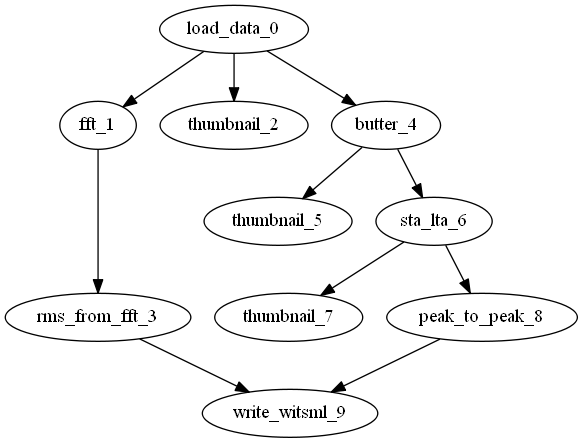
\includegraphics[width=\linewidth]{example_dot.png}
\caption{The directed graph of the commands auto-generated from the JSON description}
\label{fig:graph1}
\end{figure}

\subsection{Ingesting WITSML}
WITSML ingest
\subsection{Plotting results}
Different types of results plotting
\begin{lstlisting}
{
"figure_size" : [ 36, 12],
"dpi" : 100,
"start_of_fibre" : 0,
"end_of_fibre" : 480,
"time_reference" : "time.npy",
"depth_reference" : "measured_depth.npy",
"depth_display_unit" : "ft",
"well_segments" : "C:\\NotBackedUp\\2019scr0002\\jobInfo\\segments.txt",

"label_list" : [ 
{"event_label_start" : 200, "event_mark" : "2018-08-28 13:20:00", "event_text" : "Well Shut in" },
{"event_label_start" : 300, "event_mark" : "2018-08-28 14:09:00", "event_text" : "Open Well 1.6 bpm" },
{"event_label_start" : 400, "event_mark" : "2018-08-28 14:20:00", "event_text" : "open well 3.3 bpm" },
{"event_label_start" : 600, "event_mark" : "2018-08-28 14:21:00", "event_text" : "system stop" },
{"event_label_start" : 600, "event_mark" : "2018-08-28 14:25:00", "event_text" : "system stop" }],

"plots" : [
{
"plot_type" : "well_log",
"out_plot" : "ALL_BANDS",
"plot_list" : [ 
 { "title_text" : "Band 0", "data" : "band_0-nyquist.npy", "colormap" : "UAVK" },
 { "title_text" : "Band 1", "data" : "band_01_2-10.npy", "colormap" : "magma" },
 { "title_text" : "Band 2", "data" : "band_02_10-50.npy", "colormap" : "cividis" },
 { "title_text" : "Band 3", "data" : "band_03_50-200.npy", "colormap" : "plasma" },
 { "title_text" : "Band 4", "data" : "band_04_200-500.npy", "colormap" : "viridis" } ]
},
{
"plot_type" : "stack",
"out_plot" : "STACK",
"plot_list" : [ 
 { "title_text" : "Band 1", "data" : "band_01_2-10.npy", "colormap" : "viridis", "alpha" : "0.25"},
 { "title_text" : "Band 2", "data" : "band_02_10-50.npy", "colormap" : "plasma", "alpha" : "0.25"},
 { "title_text" : "Band 3", "data" : "band_03_50-200.npy", "colormap" : "inferno", "alpha" : "0.25"},
 { "title_text" : "Band 4", "data" : "band_04_200-500.npy", "colormap" : "magma", "alpha" : "0.25"} ]
},
{
"plot_type" : "rgb",
"out_plot" : "RGB",
"plot_list" : [ 
 { "title_text" : "Band 1", "data" : "band_01_2-10.npy", "inverted" : "yes"},
 { "title_text" : "Band 2", "data" : "band_02_10-50.npy", "inverted" : "yes"},
 { "title_text" : "Band 4", "data" : "band_04_200-500.npy", "inverted" : "yes"} ]
}
] 
}
\end{lstlisting}
